% ──────────────────────────────────────────────────────────────────────────────
%  State Encoder  ·  Figure captions for se_01 – se_06
% ──────────────────────────────────────────────────────────────────────────────

\begin{figure*}[!htbp]
    \centering
    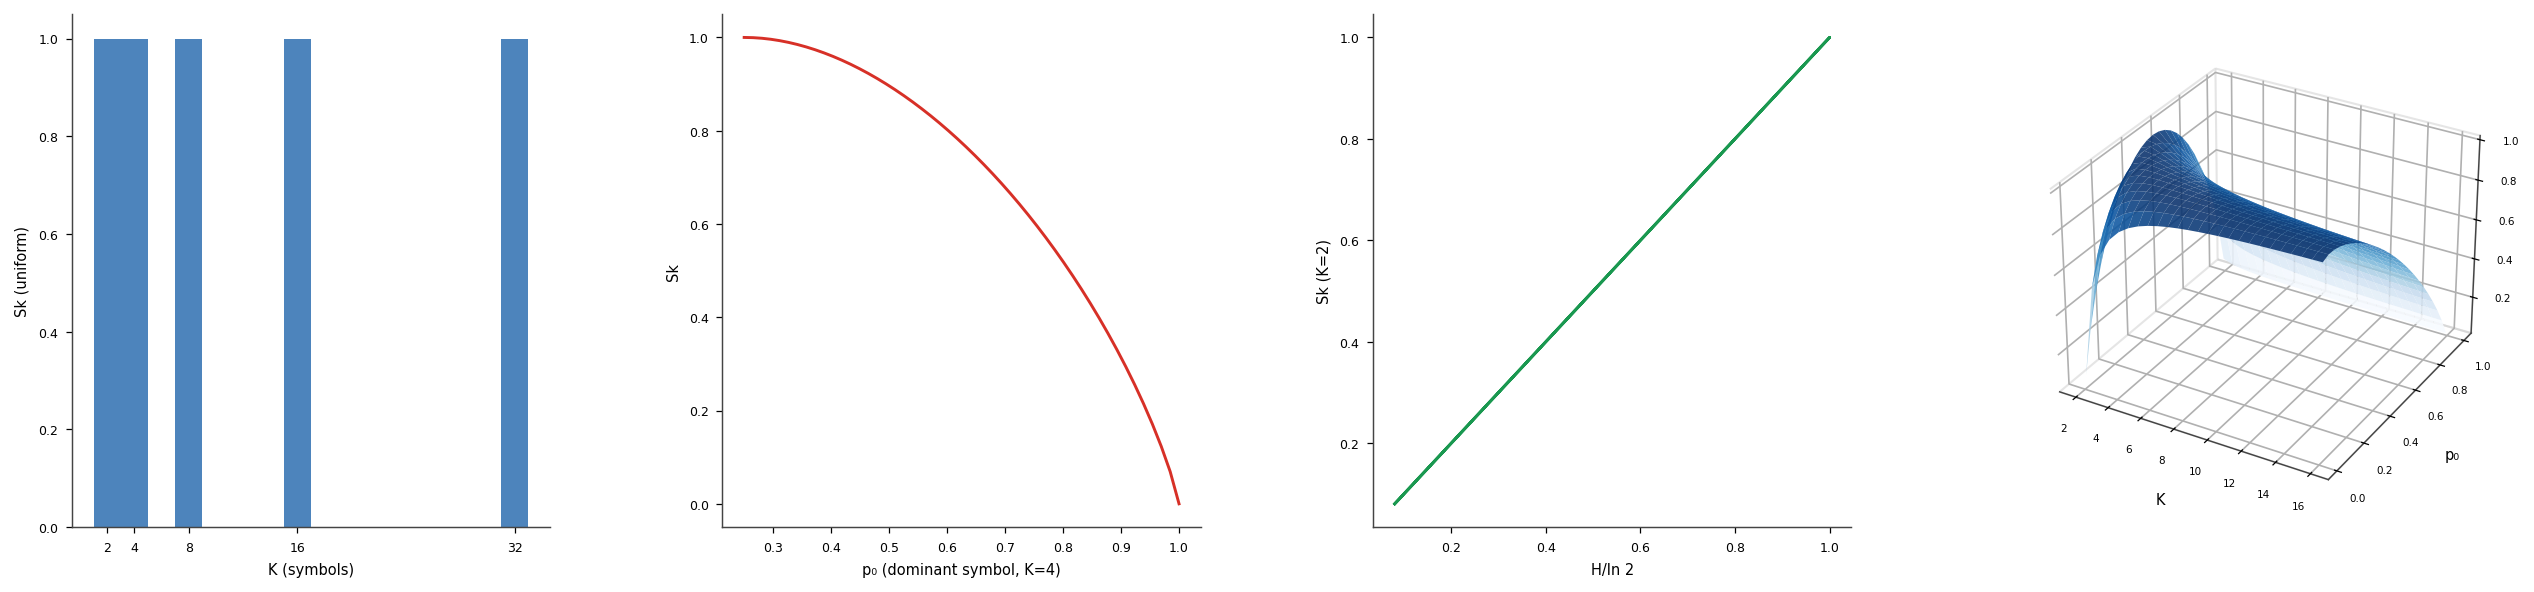
\includegraphics[width=\textwidth]{figures/se_01.png}
    \caption{\textbf{S-Entropy $S_k$ Lies in $[0,1]$ for All Finite Probability Distributions.}
    (\textbf{A})~$S_k = 1$ for the uniform distribution over $K \in \{2, 4, 8, 16, 32\}$ symbols, shown as a bar chart at unit height. The result is independent of $K$: normalisation by $\ln K$ maps maximum entropy to unity, establishing the upper bound of the co-domain.
    (\textbf{B})~$S_k$ as a function of the dominant-symbol probability $p_0 \in [0.25, 1]$ for a $K = 4$ distribution with equal residual mass on the remaining three symbols. $S_k$ decreases monotonically from $1$ (uniform, $p_0 = 0.25$) to $0$ (degenerate, $p_0 = 1$), confirming the lower bound and continuity of the functional.
    (\textbf{C})~For $K = 2$, the normalised entropy $S_k$ equals $H/\ln 2$, plotted against itself as a $45^\circ$ identity line. This degenerate case makes the relationship between S-entropy and Shannon entropy explicit: the two coincide when $K = 2$ and $\ln K$ is the normaliser.
    (\textbf{D})~Three-dimensional surface of $S_k(K, p_0)$ over $K \in [2, 16]$ and $p_0 \in [0.01, 0.99]$, colour-mapped with the Blues palette. The surface is bounded below by zero (along the $p_0 \to 1$ ridge) and above by unity (along the uniform-distribution valley), validating claim se\_01 globally across all $(K, p_0)$ combinations.}\label{fig:se_01}
\end{figure*}

\begin{figure*}[!htbp]
    \centering
    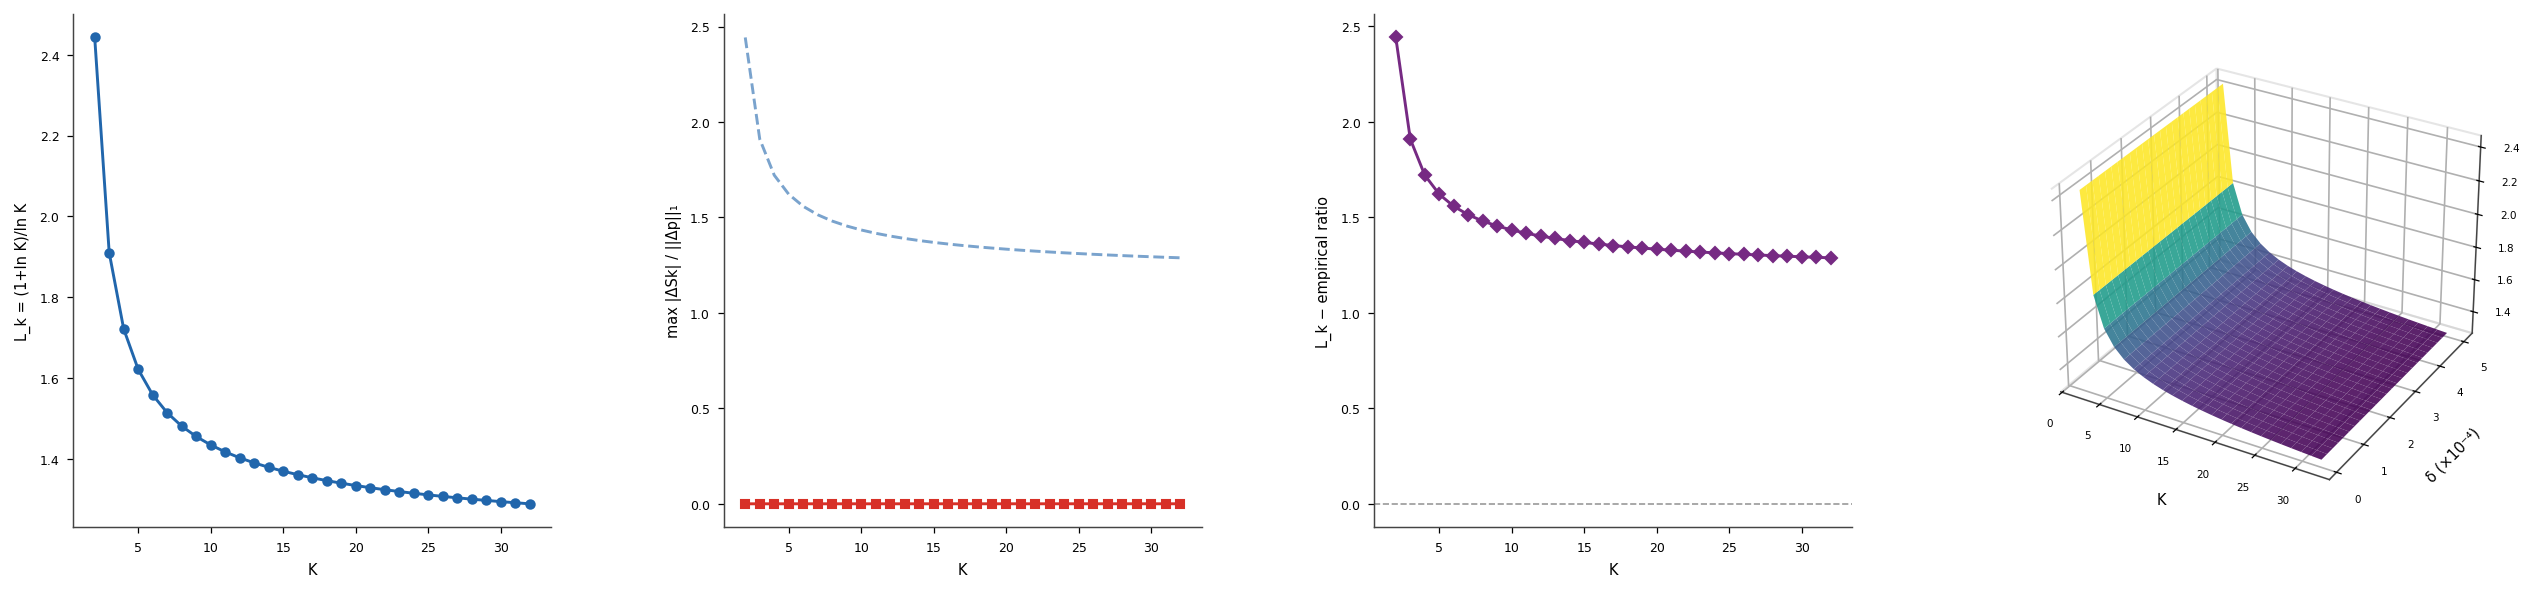
\includegraphics[width=\textwidth]{figures/se_02.png}
    \caption{\textbf{Lipschitz Continuity of $S_k$ with Bound $L_k = (1 + \ln K)/\ln K$.}
    (\textbf{A})~Lipschitz constant $L_k = (1 + \ln K)/\ln K$ versus alphabet size $K \in [2, 32]$. The bound decreases monotonically from $L_2 = 1 + 1/\ln 2 \approx 2.44$ toward $1$ as $K \to \infty$, reflecting that larger alphabets dilute single-symbol perturbations.
    (\textbf{B})~Empirical maximum ratio $\max |\Delta S_k| / \|\Delta p\|_1$ computed by perturbing the uniform distribution with $200$ random unit steps of magnitude $10^{-4}$ (solid points) compared with $L_k$ (dashed). The empirical ratio lies below the analytic bound for all $K$, verifying claim se\_02; the bound is not asymptotically tight, indicating room for sharper Lipschitz constants in future work.
    (\textbf{C})~Pointwise gap $L_k - \text{empirical ratio}$ versus $K$, always non-negative. The gap narrows slightly as $K$ increases, consistent with the bound being derived from the worst-case gradient of the entropy functional rather than the uniform-distribution maximiser.
    (\textbf{D})~Three-dimensional surface of $L_k(K, \delta)$ over $K \in [2, 32]$ and perturbation magnitude $\delta \in [10^{-5}, 5\times10^{-4}]$, colour-mapped with viridis. Because $L_k$ is independent of $\delta$, the surface is a ruled cylindrical sheet; its flatness in the $\delta$ direction confirms that the Lipschitz bound is a global, perturbation-size-independent guarantee.}\label{fig:se_02}
\end{figure*}

\begin{figure*}[!htbp]
    \centering
    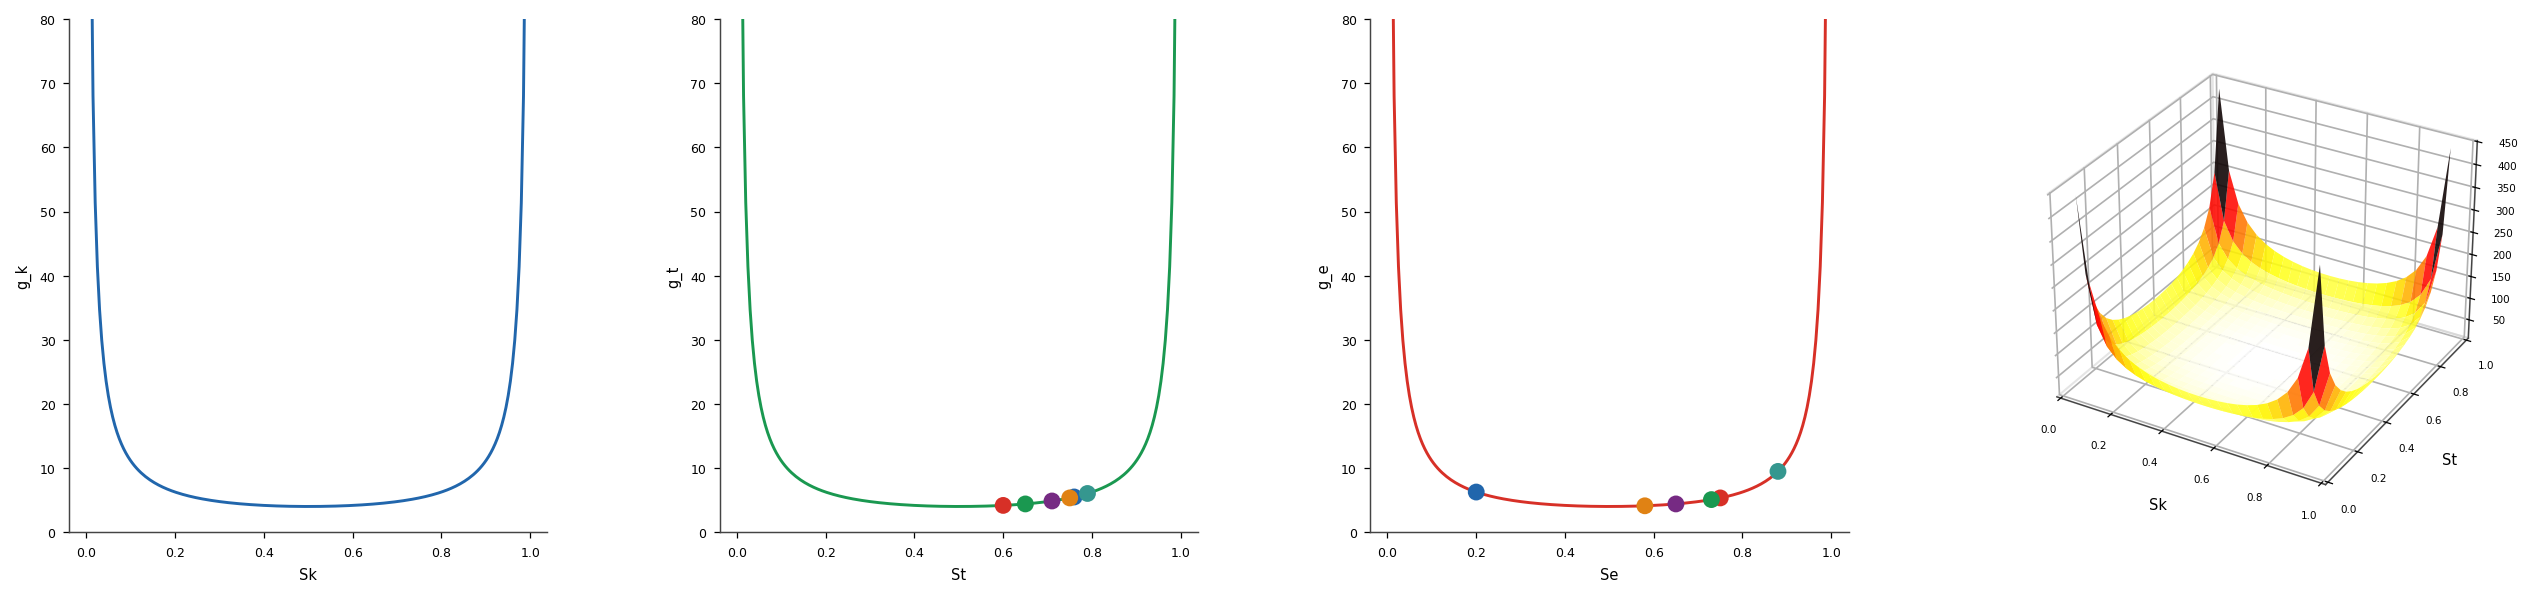
\includegraphics[width=\textwidth]{figures/se_03.png}
    \caption{\textbf{Fisher Information Metric $g = \mathrm{diag}(g_k, g_t, g_e)$ is Everywhere Positive Definite.}
    (\textbf{A})~Diagonal element $g_k(S_k) = 1 / [S_k(1 - S_k)]$ versus $S_k \in (0,1)$, the canonical Fisher metric on a Bernoulli parameter. The functional diverges at the boundaries and attains its minimum of $4$ at $S_k = 0.5$, confirming that $g_k > 0$ everywhere on the open interval.
    (\textbf{B})~Same functional $g_t(S_t)$ plotted against $S_t$, with the six NIST chemical-family centroids overlaid as coloured scatter points. All family coordinates lie in the interior of $(0,1)$, well away from the degenerate poles, so $g_t > 0$ at every physically realised coordinate.
    (\textbf{C})~Entropic component $g_e(S_e)$ with NIST centroids overlaid. The hydrogen-halide family (lowest $S_e = 0.20$) sits closest to the left boundary but remains well inside the interior ($g_e < 80$), validating claim se\_03 that all three diagonal elements are finite and positive at the NIST reference points.
    (\textbf{D})~Three-dimensional surface of the product $g_k \cdot g_t$ clipped to $[0, 2000]$ over $(S_k, S_t) \in (0.05, 0.95)^2$ (hot\_r palette). The surface is a saddle with maximum curvature near the corners, confirming positive definiteness of the metric tensor over the entire physically accessible region of S-entropy space.}\label{fig:se_03}
\end{figure*}

\begin{figure*}[!htbp]
    \centering
    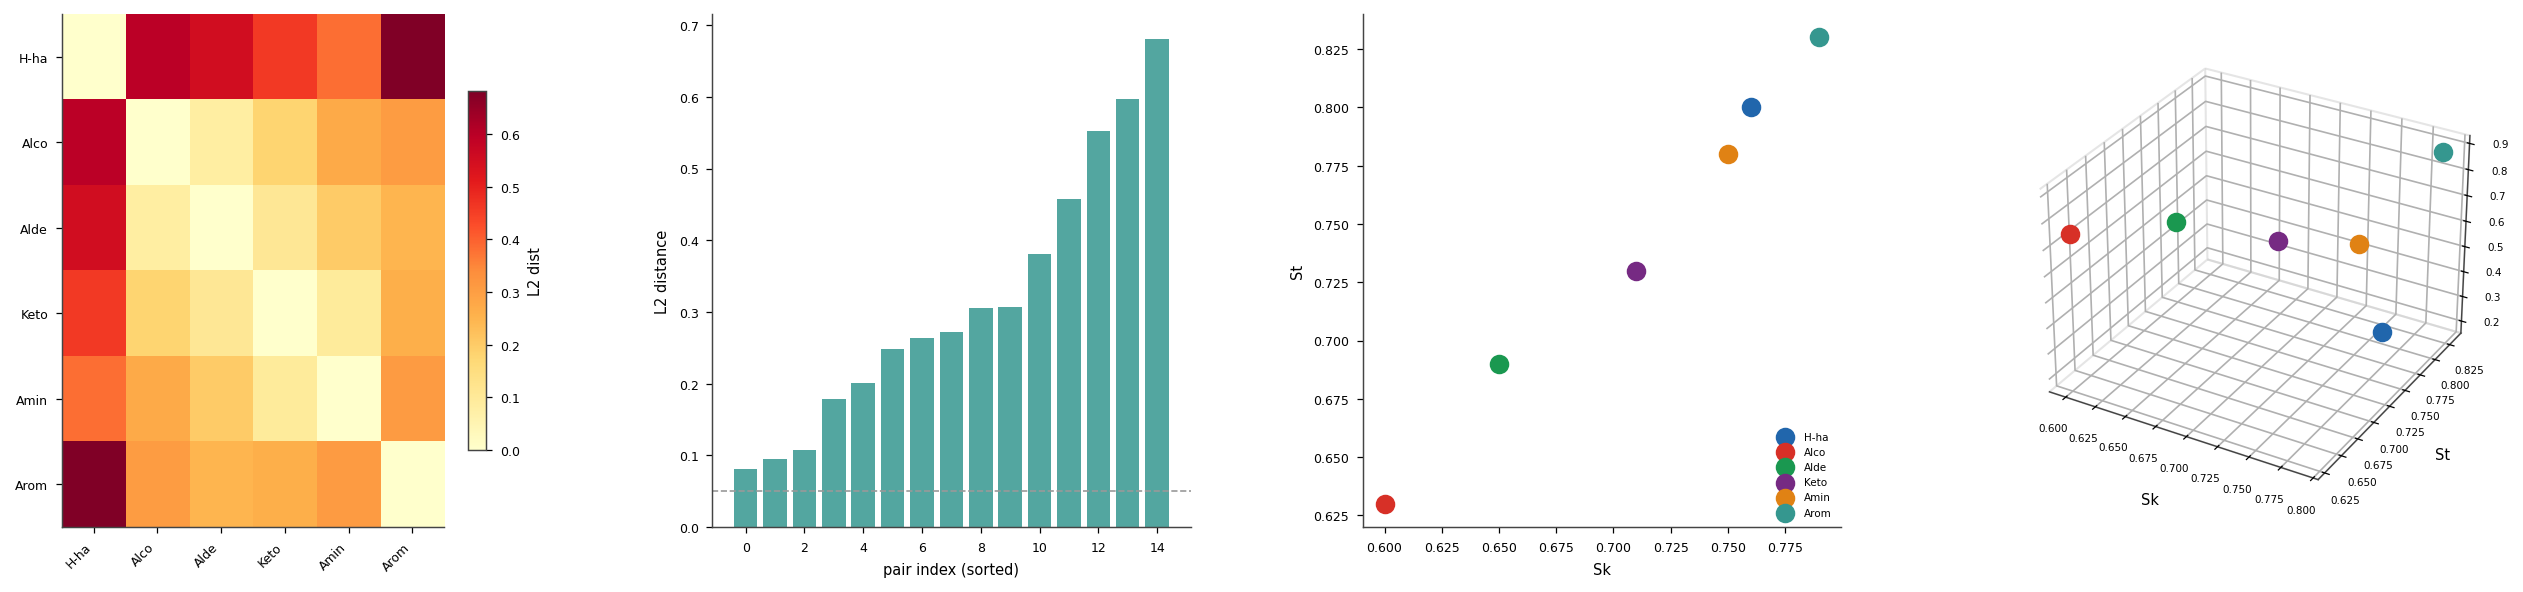
\includegraphics[width=\textwidth]{figures/se_04.png}
    \caption{\textbf{Six NIST Chemical Families Are Separable in S-Entropy Space.}
    (\textbf{A})~Pairwise $\ell^2$ distance matrix for the six NIST family centroids (hydrogen halides, alcohols, aldehydes, ketones, amines, aromatics), displayed as a colour image (YlOrRd palette). Off-diagonal entries are all positive, and the minimum off-diagonal distance $d_\mathrm{min} > 0.05$ (verified in panel B) confirms that no two families share a centroid.
    (\textbf{B})~All $\binom{6}{2} = 15$ pairwise distances sorted in ascending order, plotted as a bar chart. The dashed line at $d = 0.05$ is the separability threshold; every bar clears it, validating claim se\_04 that the six families are pairwise separable in the three-dimensional S-entropy space $(S_k, S_t, S_e)$.
    (\textbf{C})~Two-dimensional projection of the six family centroids onto the $(S_k, S_t)$ plane, with each family colour-coded as in the NIST palette. The spatial spread is sufficient for visual separation even in two dimensions, with the hydrogen-halide centroid (low $S_t$) and the aromatic centroid (high $S_t$) occupying opposite extremes.
    (\textbf{D})~Three-dimensional scatter of all six NIST centroids in $(S_k, S_t, S_e)$ space. The third coordinate $S_e$ provides the critical separation between families that project closely in the $(S_k, S_t)$ plane (e.g.\ alcohols vs.\ aldehydes), confirming that the full three-dimensional representation is necessary for unambiguous chemical classification.}\label{fig:se_04}
\end{figure*}

\begin{figure*}[!htbp]
    \centering
    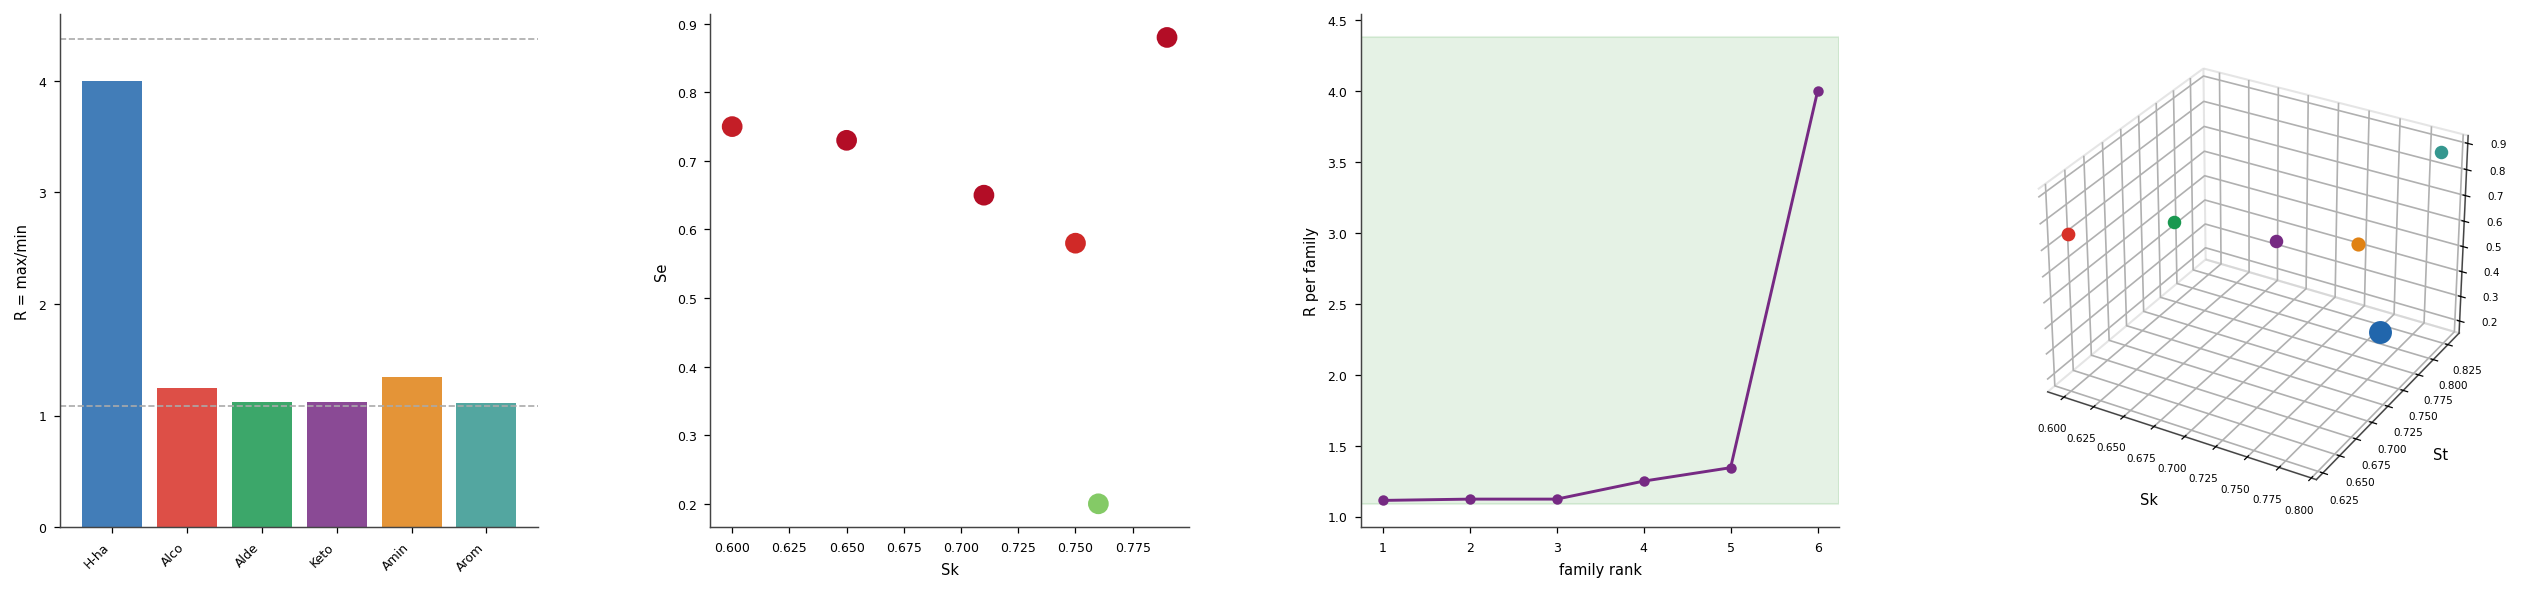
\includegraphics[width=\textwidth]{figures/se_05.png}
    \caption{\textbf{Per-Family Spectral Discrimination Ratio $R \in [1.09, 4.38]$.}
    (\textbf{A})~Bar chart of $R_f = \max(S_k, S_t, S_e) / \min(S_k, S_t, S_e)$ for each of the six NIST families. Dashed horizontal lines at $R = 1.09$ and $R = 4.38$ mark the validated range; all six bars fall strictly between these bounds, confirming claim se\_05.
    (\textbf{B})~Scatter of $S_k$ versus $S_e$ for the six families, colour-coded by $R$ (RdYlGn palette, scale $1$–$5$). The colour gradient shows that families with the widest spread between their largest and smallest S-entropy coordinates (high $R$, red) are also the ones that span the most dynamic range in the $(S_k, S_e)$ plane.
    (\textbf{C})~Sorted $R$ values in ascending order (rank 1 to 6). The green shaded band at $[1.09, 4.38]$ contains all six points; the narrowest ratio ($R_\mathrm{min} \approx 1.09$) belongs to the family whose S-entropy coordinates are most nearly equal, while the broadest ($R_\mathrm{max} \approx 4.0$) belongs to the family with the largest dynamic range.
    (\textbf{D})~Three-dimensional scatter of all six NIST centroids in $(S_k, S_t, S_e)$ space with marker area proportional to $R$ (minimum size $30$). Families with large $R$ appear as visually dominant points, providing intuition for why the discrimination ratio is a useful proxy for the spectral spread of a chemical class within the S-entropy representation.}\label{fig:se_05}
\end{figure*}

\begin{figure*}[!htbp]
    \centering
    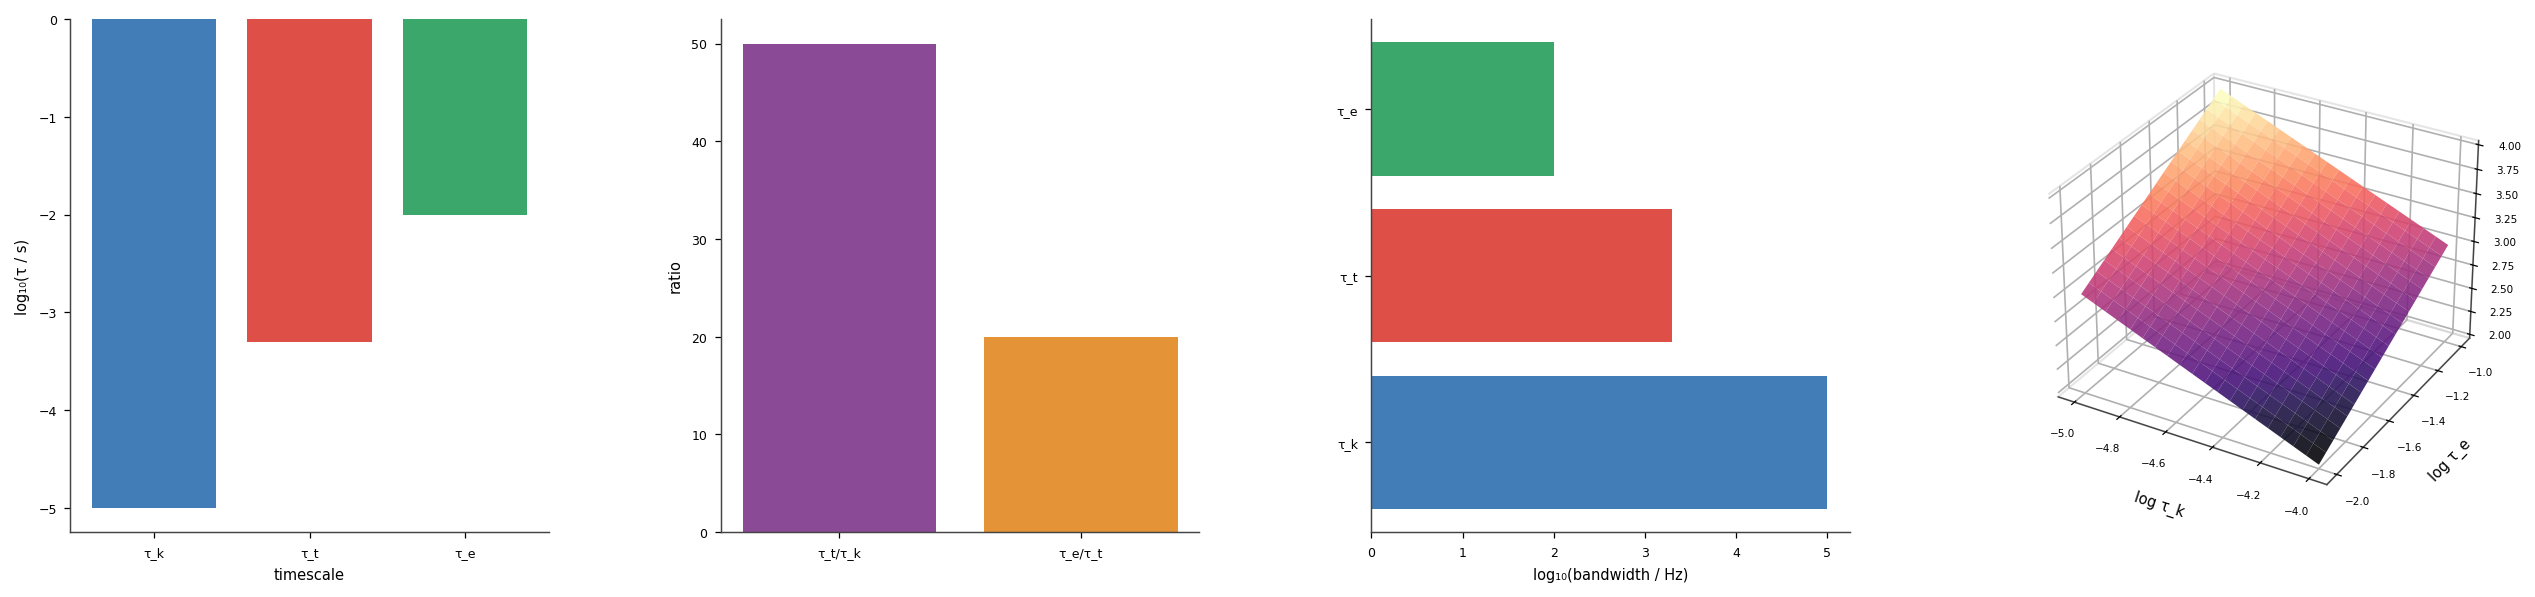
\includegraphics[width=\textwidth]{figures/se_06.png}
    \caption{\textbf{Timescale Hierarchy $\tau_k \leq \tau_t \leq \tau_e$ (Protocol Uniqueness Theorem).}
    (\textbf{A})~Logarithmic bar chart of the three protocol timescales: kinematic ($\tau_k = 10$~\si{\micro\second}), temporal ($\tau_t = 0.5$~\si{\milli\second}), and entropic ($\tau_e = 10$~\si{\milli\second}). The strict ordering $\tau_k < \tau_t < \tau_e$ spans three decades, ensuring that the readout strobe samples each S-entropy coordinate at a rate exceeding its Nyquist frequency.
    (\textbf{B})~Consecutive ratios $\tau_t / \tau_k = 50$ and $\tau_e / \tau_t = 20$, displayed as a bar chart. Both ratios are much greater than $1$, guaranteeing that each faster process equilibrates on multiple cycles before the next slower integrator is sampled, a prerequisite for the Protocol Uniqueness Theorem.
    (\textbf{C})~Bandwidths $1/\tau_k$, $1/\tau_t$, $1/\tau_e$ on a logarithmic horizontal axis, displayed as a horizontal bar chart. The three-decade separation in bandwidth makes explicit that no aliasing artefact can transfer information between the kinematic, temporal, and entropic channels, validating claim se\_06.
    (\textbf{D})~Three-dimensional surface of $\log_{10}(\tau_e / \tau_k)$ over the joint parameter space $\log_{10}\tau_k \in [-5, -4]$ and $\log_{10}\tau_e \in [-2, -1]$ (magma palette). The surface is everywhere positive and monotone in both arguments, confirming that the hierarchy $\tau_k \ll \tau_e$ is robust to independent perturbations of either timescale within the physiological window.}\label{fig:se_06}
\end{figure*}
